%Begin the document and set up the style of the document
\documentclass[a4paper]{article}

% Install the required packages for the document 
\usepackage{envmath}
\usepackage{esvect}
\usepackage{graphicx}
\usepackage{gensymb}
\usepackage{tikz}
\usepackage[mathcal]{euscript}
\usepackage{geometry}
\usepackage{enumitem}
\usepackage{mathtools}
\usepackage{graphicx}
\usepackage{amsmath}
\usepackage{amscd}
\usepackage{amssymb}
\usepackage{amsfonts}
\usepackage{harpoon}
\usepackage{pgf}
\usepackage{tikz}
\usepackage{mathrsfs}
\usepackage{asyalign}
\usepackage{physics}
\usepackage{enumitem}
\usepackage{xhfill}
\usepackage{accents}
\usepackage{cite}
\usepackage{url}
\usepackage[tableposition=top]{caption}
\usepackage{ifthen}
\usepackage[utf8]{inputenc}
\usepackage{tikz-3dplot}
\usetikzlibrary{patterns}
\usetikzlibrary{arrows}

% Page and style settings
\parskip=8pt
\parindent=0pt
% Right margin
\textwidth=6.25in
% Left margin
\oddsidemargin=0pt
\evensidemargin=0pt
% Bottom margin
\textheight=10in
% Top margin
\topmargin=-0.75in
\baselineskip=11pt
% end of page and other style settings

\renewcommand{\familydefault}{\sfdefault}


% Begin the text of the document
\begin{document}

% Begin the Title Page
\begin{titlepage}

\newcommand{\HRule}{\rule{\linewidth}{0.5mm}} % Defines a new command for the horizontal lines, change thickness here

\center % Center everything on the page
 
\textsc{\LARGE University of Sydney}\\[1.5cm] % Name of your university/college
\textsc{\Large MATH 1906}\\[0.5cm] % Major heading such as course name
\textsc{\large SSP}\\[0.5cm] % Minor heading such as course title

\HRule \\[0.4cm]
{ \huge \bfseries Assignment 2 - Fractals}\\[0.4cm] % Title of your document
\HRule \\[1.5cm]

\begin{minipage}{0.4\textwidth}
\begin{flushleft} \large
\emph{Author:}
Keegan Gyoery % Your name
\\
\emph{SID:}
470413467
\end{flushleft}
\end{minipage}
~
\begin{minipage}{0.4\textwidth}
\begin{flushright} \large
\emph{Tutor:} 
Florica C. Cirstea % Tutor's Name
\\
\emph{Tutorial:}
New Law Annexe SR 442, Monday 4pm
\end{flushright}
\end{minipage}\\[4cm]

{\large \today}\\[3cm] % Date, change the \today to a set date if you want to be precise

\vfill % Fill the rest of the page with whitespace

\end{titlepage}

\pagenumbering{arabic}
%%%%%%%%%%%%%%%%%%%%%%%%%%%
%%%%%%%%%%%%%%%%%%%%%%%%%%%
%%%%%%%%%%%%%%%%%%%%%%%%%%%
%%%%%%%%%%%%%%%%%%%%%%%%%%%

\begin{enumerate}[label=\textbf{\arabic*.}]
	\item

	\begin{enumerate}
		\item Using the given initator and the generative steps to construct the fractal, we can construct the second, third and fourth iterations of the fractal, as seen below.


		The following figure is Iteration 2.

		\begin{center}
		\begin{figure}[h!]
			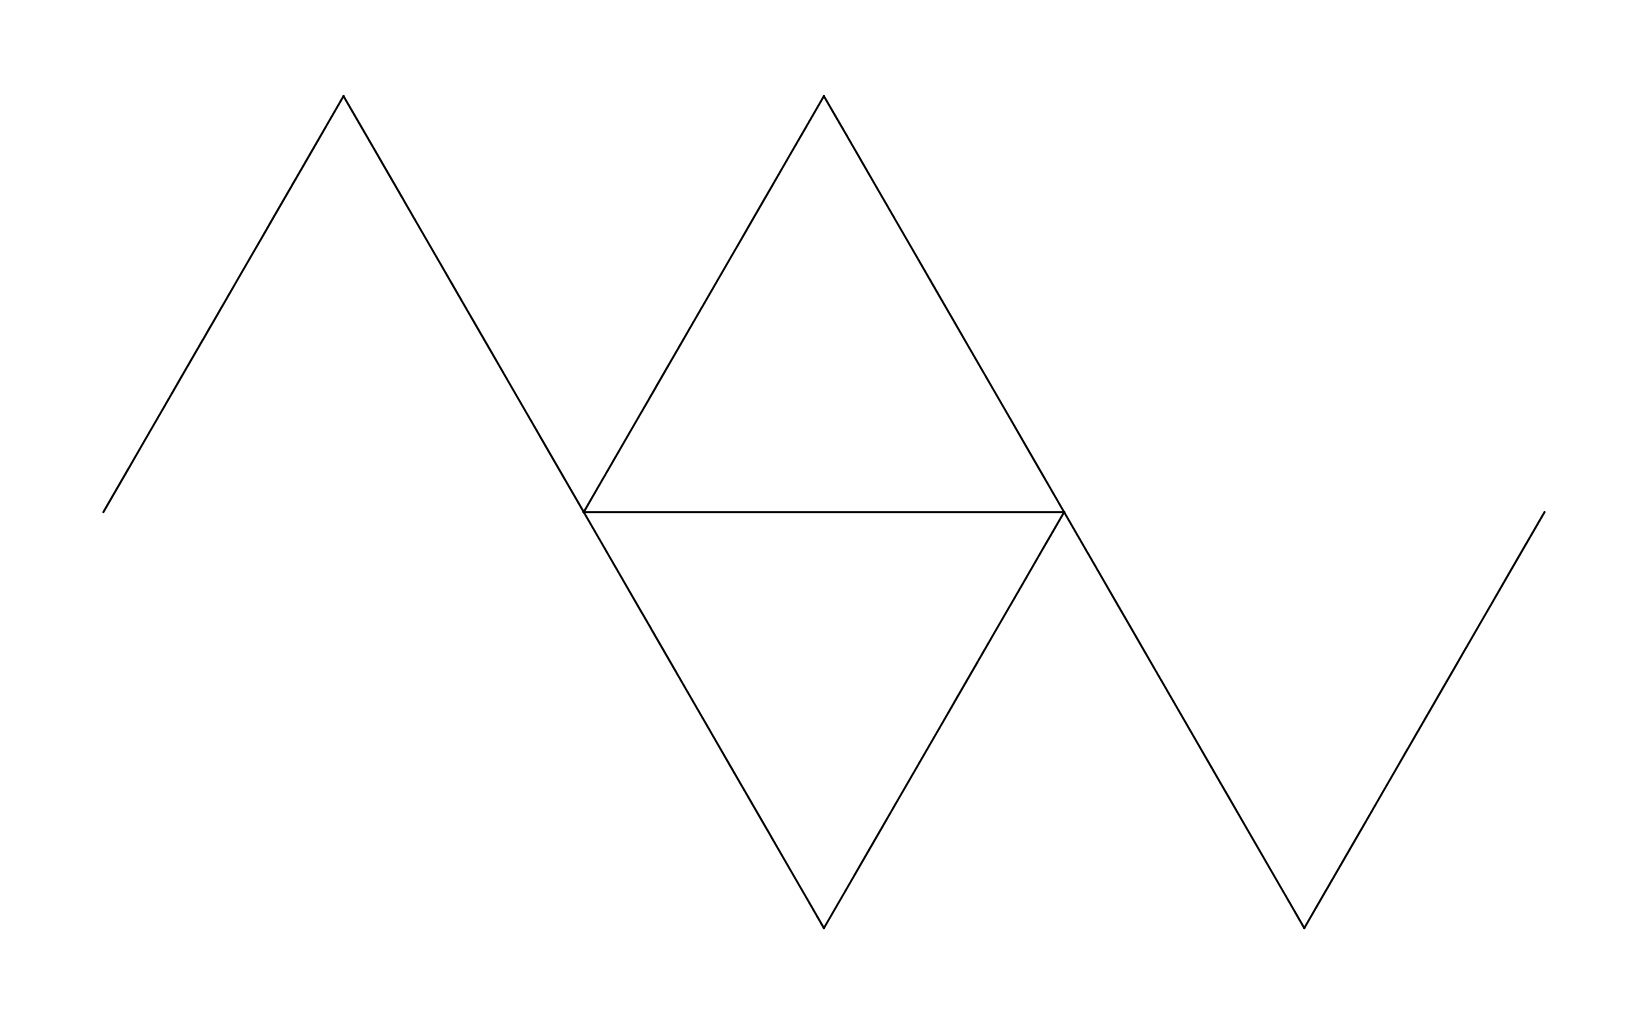
\includegraphics[width=\linewidth]{IFS2_S.png}
		\end{figure}
		\end{center}

		\bigbreak

		The following figure is Iteration 3.

		\begin{center}
		\begin{figure}[h!]
			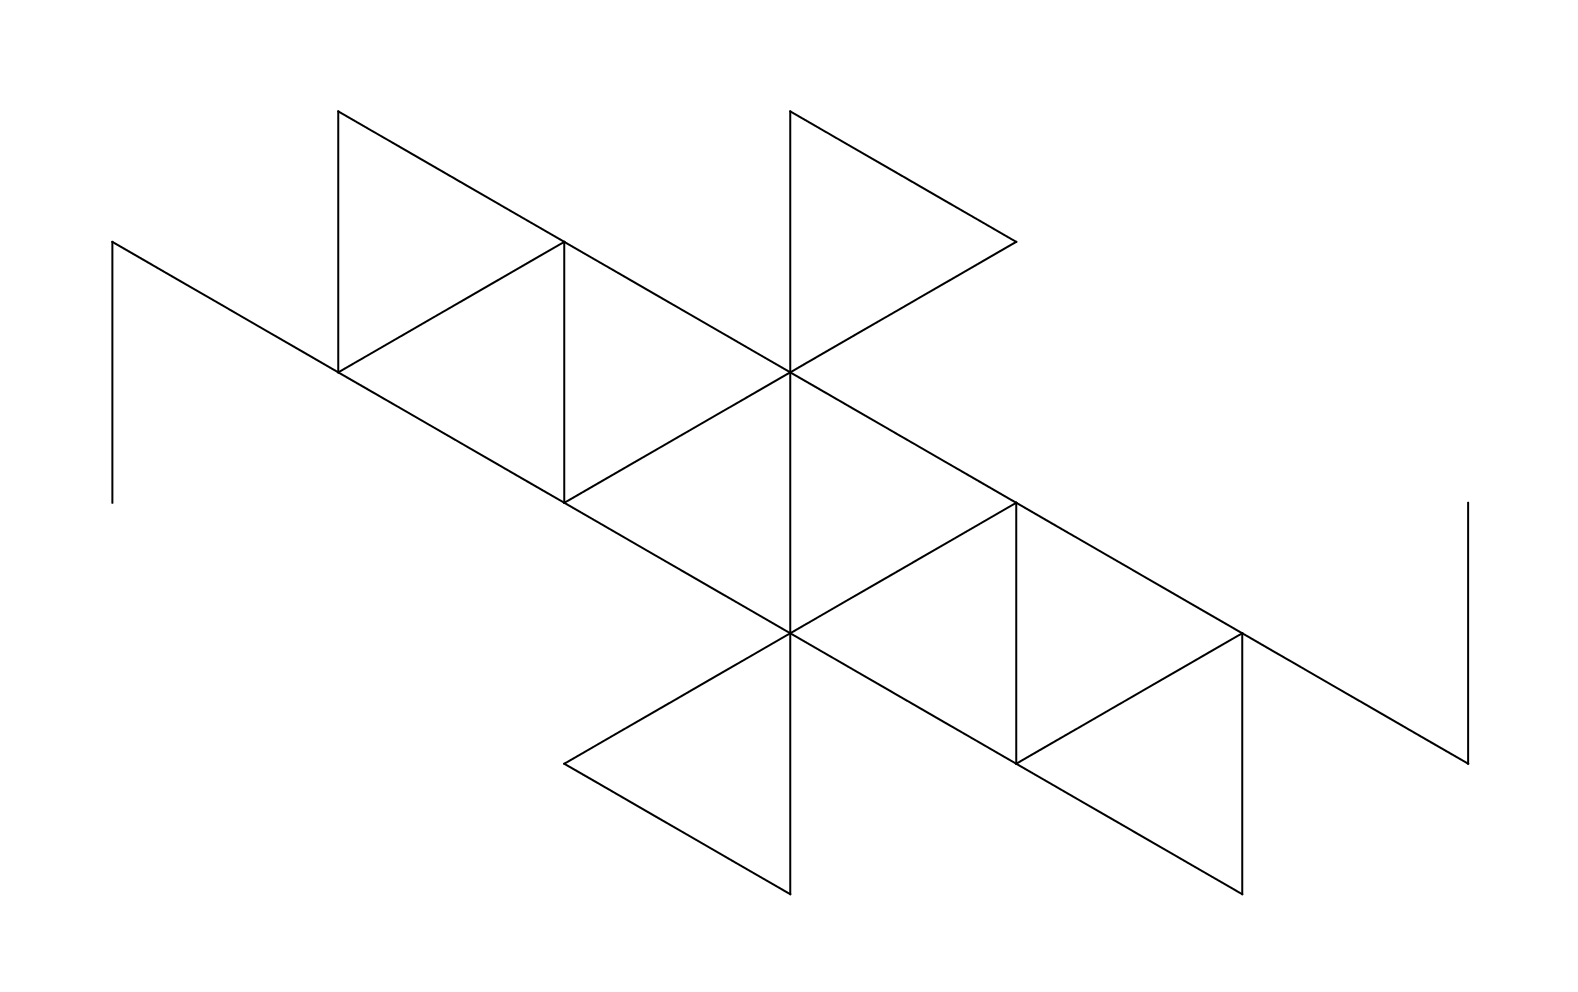
\includegraphics[width=\linewidth]{IFS3_S.png}
		\end{figure}
		\end{center}

		\bigbreak

		\pagebreak

		The following figure is Iteration 4, and is the final iteration we are to construct.

		\begin{figure}[h!]
			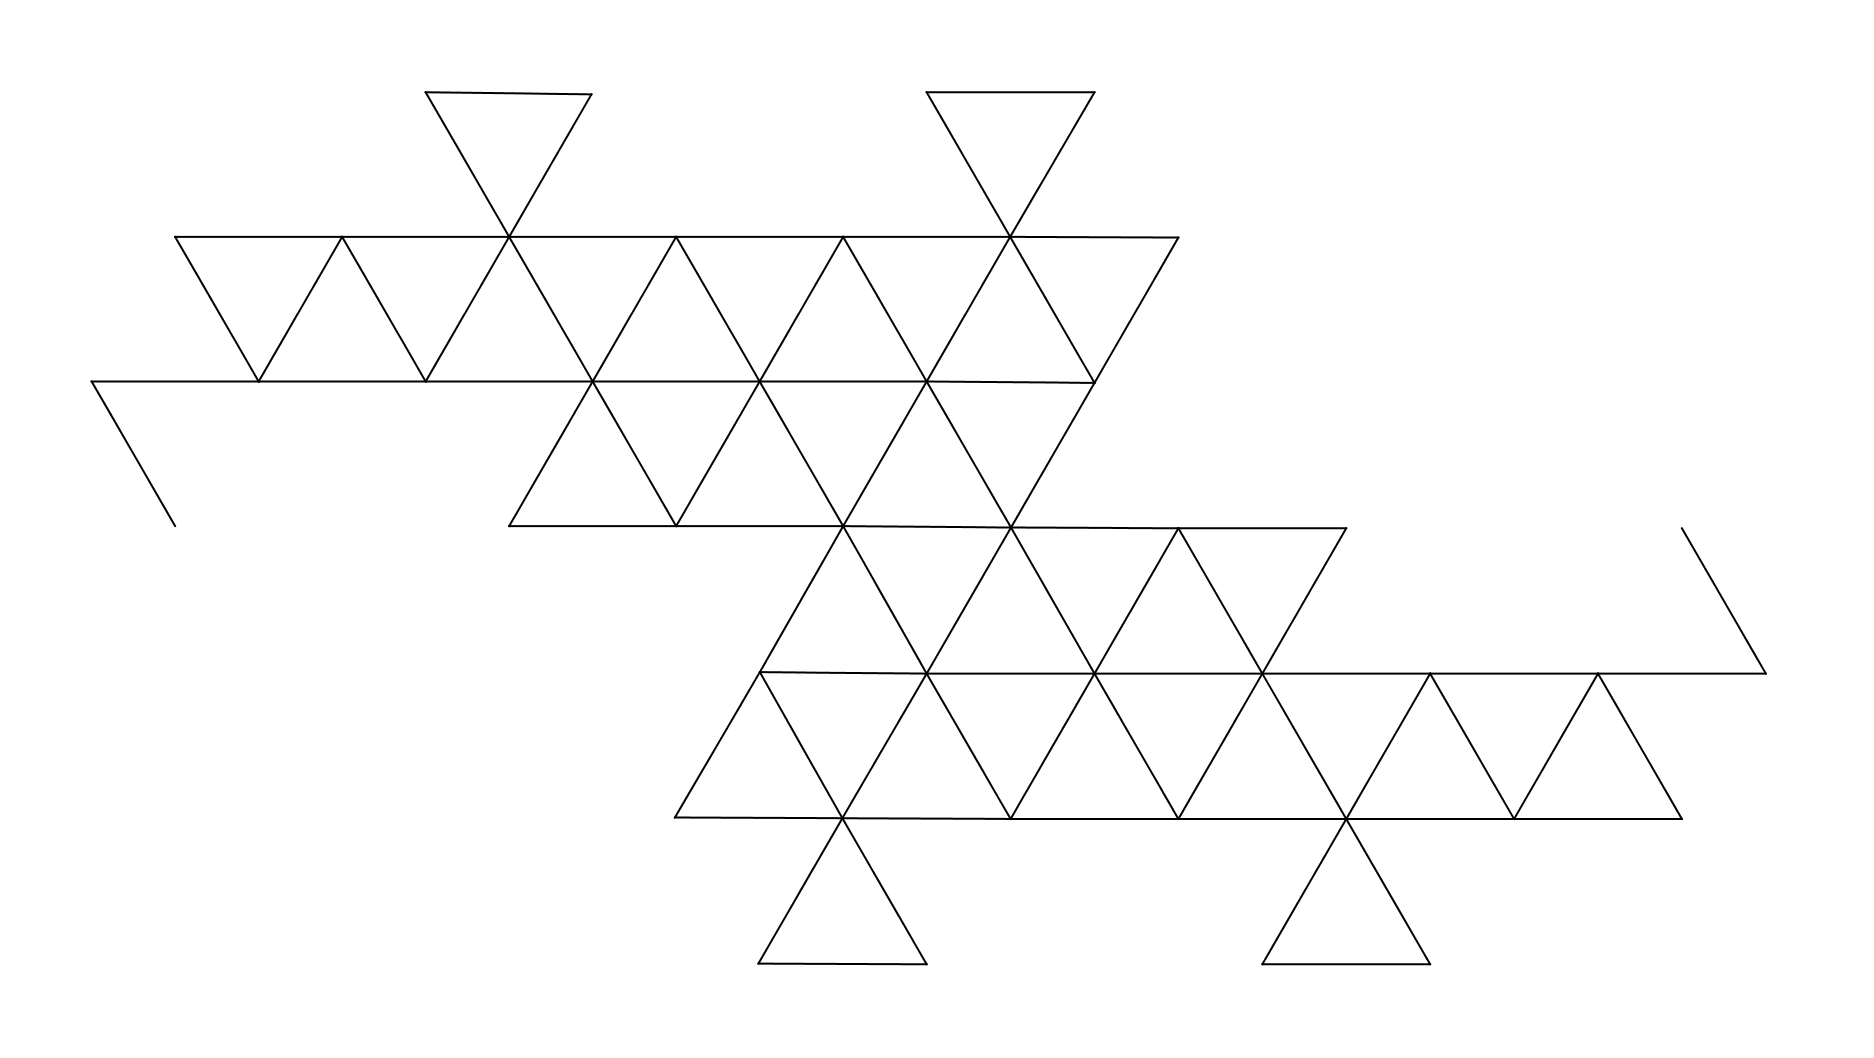
\includegraphics[width=\linewidth]{IFS4_S.png}
		\end{figure}

		\bigbreak

		\item The similarity dimension of a fractal is calculated using the following formula:

		\begin{align*}
		d_{ss} & = \frac{\log{N}}{\log{\frac{1}{r}}}\\
		\end{align*}

		where $d_{ss}$ is the self similarity dimension, $N$ is the number of copies of the initiator, and $r$ is the scaling factor. Applying this formula to our fractal, $N = 3$, and $r = \frac{1}{\sqrt{3}}$. Thus calculating the self similarity dimension of our fractal gives:

		\begin{align*}
		d_{ss} & = \frac{\log{N}}{\log{\frac{1}{r}}}\\
		& = \frac{\log{3}}{\log{\frac{1}{\frac{1}{\sqrt{3}}}}}\\
		& = \frac{\log{3}}{\log{\sqrt{3}}}\\
		& = \frac{\log{3}}{\frac{1}{2}\log{3}}\\
		& = \frac{1}{\frac{1}{2}}\\
		\therefore d_{ss} & = 2\\
		\end{align*}

		\pagebreak

		\item In order to calculate the IFS for the fractal given, we must examine the transformation of each of three copies from the initiator, as this process will be iteratively applied at every step. Examining the first line segment of the three that result in the first iteration of the fractal, we arrive at the following transformations.

		\bigbreak

		\begin{center}
		Scaling by a factor of $\frac{1}{\sqrt{3}}$.
		\end{center}

		\begin{align*}
		f(x,y) & \rightarrow f_1(x^{\prime},y^{\prime})\\
		x & \rightarrow x^{\prime}\\
		& \rightarrow \frac{x}{\sqrt{3}}\\
		\therefore x^{\prime} & = \frac{x}{\sqrt{3}}\\
		y & \rightarrow y^{\prime}\\
		& \rightarrow \frac{y}{\sqrt{3}}\\
		\therefore y^{\prime} & = \frac{y}{\sqrt{3}}\\
		\end{align*}

		\begin{center}
		Rotation by $\frac{\pi}{6}$.
		\end{center}

		\begin{equation*}
		f_1(x^{\prime},y^{\prime}) \rightarrow f_1(x^{\prime \prime},y^{\prime \prime})\\
		\end{equation*}

		\begin{equation*}
		\begin{bmatrix*}[r]
			\hspace{1mm} \cos{\theta} & -\sin{\theta} \hspace{1mm}\\
			\hspace{1mm} \sin{\theta} & \cos{\theta} \hspace{1mm}\\
		\end{bmatrix*}
		\begin{bmatrix*}[r]
			\hspace{1mm} x^{\prime} \hspace{1mm}\\
			\hspace{1mm} y^{\prime} \hspace{1mm}\\
		\end{bmatrix*}
		=
		\begin{bmatrix*}[r]
			\hspace{1mm} x^{\prime \prime} \hspace{1mm}\\
			\hspace{1mm} y^{\prime \prime} \hspace{1mm}\\
		\end{bmatrix*}
		\end{equation*}

		\begin{equation*}
		\begin{bmatrix*}[r]
			\hspace{1mm} \cos{\frac{\pi}{6}} & -\sin{\frac{\pi}{6}} \hspace{1mm}\\
			\hspace{1mm} \sin{\frac{\pi}{6}} & \cos{\frac{\pi}{6}} \hspace{1mm}\\
		\end{bmatrix*}
		\begin{bmatrix*}[r]
			\hspace{1mm} \frac{x}{\sqrt{3}} \hspace{1mm}\\
			\hspace{1mm} \frac{y}{\sqrt{3}} \hspace{1mm}\\
		\end{bmatrix*}
		=
		\begin{bmatrix*}[r]
			\hspace{1mm} x^{\prime \prime} \hspace{1mm}\\
			\hspace{1mm} y^{\prime \prime} \hspace{1mm}\\
		\end{bmatrix*}
		\end{equation*}

		\begin{equation*}
		\begin{bmatrix*}[r]
			\hspace{1mm} \frac{\sqrt{3}}{2} & -\frac{1}{2} \hspace{1mm}\\
			\hspace{1mm} \frac{1}{2} & \frac{\sqrt{3}}{2} \hspace{1mm}\\
		\end{bmatrix*}
		\begin{bmatrix*}[r]
			\hspace{1mm} \frac{x}{\sqrt{3}} \hspace{1mm}\\
			\hspace{1mm} \frac{y}{\sqrt{3}} \hspace{1mm}\\
		\end{bmatrix*}
		=
		\begin{bmatrix*}[r]
			\hspace{1mm} \frac{x}{2} - \frac{y}{2\sqrt{3}} \hspace{1mm}\\
			\hspace{1mm} \frac{x}{2\sqrt{3}} + \frac{y}{2} \hspace{1mm}\\
		\end{bmatrix*}
		\end{equation*}

		\begin{align*}
		\therefore x^{\prime \prime} & = \frac{x}{2} - \frac{y}{2\sqrt{3}}\\
		\therefore x^{\prime \prime} & = \frac{\sqrt{3}x-y}{2\sqrt{3}}\\
		\therefore y^{\prime \prime} & = \frac{x}{2\sqrt{3}} + \frac{y}{2}\\
		\therefore y^{\prime \prime} & = \frac{x + \sqrt{3}y}{2\sqrt{3}}\\
		\end{align*}

		There is no Translation for the first segment. Thus the map for the first segment is given by the following map.

		\begin{align*}
		f(x,y) & \rightarrow f_1(x^{\prime \prime},y^{\prime \prime})\\
		f_1(x^{\prime \prime},y^{\prime \prime})& = f_1(x_1,y_1)\\
		\therefore f(x,y) & \rightarrow f_1(x_1,y_1)\\
		\therefore f(x,y) & \rightarrow f_1\left(\frac{3x-\sqrt{3}y}{6},\frac{\sqrt{3}x + 3y}{6}\right)\\
		\end{align*}

		\pagebreak

		Examining the second line segment of the three that result in the first iteration of the fractal, we arrive at the following transformations.

		\bigbreak

		\begin{center}
		Scaling by a factor of $\frac{1}{\sqrt{3}}$.
		\end{center}

		\begin{align*}
		f(x,y) & \rightarrow f_2(x^{\prime},y^{\prime})\\
		x & \rightarrow x^{\prime}\\
		& \rightarrow \frac{x}{\sqrt{3}}\\
		\therefore x^{\prime} & = \frac{x}{\sqrt{3}}\\
		y & \rightarrow y^{\prime}\\
		& \rightarrow \frac{y}{\sqrt{3}}\\
		\therefore y^{\prime} & = \frac{y}{\sqrt{3}}\\
		\end{align*}

		\begin{center}
		Rotation by $-\frac{\pi}{2}$.
		\end{center}

		\begin{equation*}
		f_2(x^{\prime},y^{\prime}) \rightarrow f_2(x^{\prime \prime},y^{\prime \prime})\\
		\end{equation*}

		\begin{equation*}
		\begin{bmatrix*}[r]
			\hspace{1mm} \cos{\theta} & -\sin{\theta} \hspace{1mm}\\
			\hspace{1mm} \sin{\theta} & \cos{\theta} \hspace{1mm}\\
		\end{bmatrix*}
		\begin{bmatrix*}[r]
			\hspace{1mm} x^{\prime} \hspace{1mm}\\
			\hspace{1mm} y^{\prime} \hspace{1mm}\\
		\end{bmatrix*}
		=
		\begin{bmatrix*}[r]
			\hspace{1mm} x^{\prime \prime} \hspace{1mm}\\
			\hspace{1mm} y^{\prime \prime} \hspace{1mm}\\
		\end{bmatrix*}
		\end{equation*}

		\begin{equation*}
		\begin{bmatrix*}[r]
			\hspace{1mm} \cos{\left(-\frac{\pi}{2}\right)} & -\sin{\left(-\frac{\pi}{2}\right)} \hspace{1mm}\\
			\hspace{1mm} \sin{\left(-\frac{\pi}{2}\right)} & \cos{\left(-\frac{\pi}{2}\right)} \hspace{1mm}\\
		\end{bmatrix*}
		\begin{bmatrix*}[r]
			\hspace{1mm} \frac{x}{\sqrt{3}} \hspace{1mm}\\
			\hspace{1mm} \frac{y}{\sqrt{3}} \hspace{1mm}\\
		\end{bmatrix*}
		=
		\begin{bmatrix*}[r]
			\hspace{1mm} x^{\prime \prime} \hspace{1mm}\\
			\hspace{1mm} y^{\prime \prime} \hspace{1mm}\\
		\end{bmatrix*}
		\end{equation*}

		\begin{equation*}
		\begin{bmatrix*}[r]
			\hspace{1mm} 0 & 1 \hspace{1mm}\\
			\hspace{1mm} -1 & 0 \hspace{1mm}\\
		\end{bmatrix*}
		\begin{bmatrix*}[r]
			\hspace{1mm} \frac{x}{\sqrt{3}} \hspace{1mm}\\
			\hspace{1mm} \frac{y}{\sqrt{3}} \hspace{1mm}\\
		\end{bmatrix*}
		=
		\begin{bmatrix*}[r]
			\hspace{1mm} \frac{y}{\sqrt{3}} \hspace{1mm}\\
			\hspace{1mm} -\frac{x}{\sqrt{3}} \hspace{1mm}\\
		\end{bmatrix*}
		\end{equation*}

		\begin{align*}
		\therefore x^{\prime \prime} & = \frac{y}{\sqrt{3}}\\
		\therefore y^{\prime \prime} & = -\frac{x}{\sqrt{3}}\\
		\end{align*}

		\pagebreak

		\begin{center}
		Translation by $\left(\frac{1}{2},\frac{1}{2\sqrt{3}}\right)$.
		\end{center}

		\begin{align*}
		f_2(x^{\prime \prime},y^{\prime \prime}) & \rightarrow f_2(x^{\prime \prime \prime},y^{\prime \prime \prime})\\
		x^{\prime \prime} & \rightarrow x^{\prime \prime \prime}\\
		& \rightarrow \frac{y}{\sqrt{3}} + \frac{1}{2}\\
		\therefore x^{\prime \prime \prime} & = \frac{y}{\sqrt{3}} + \frac{1}{2}\\
		\therefore x^{\prime \prime \prime} & = \frac{\sqrt{3} + 2y}{2\sqrt{3}}\\
		y^{\prime \prime} & \rightarrow y^{\prime \prime \prime}\\
		& \rightarrow \frac{1}{2\sqrt{3}} - \frac{x}{\sqrt{3}}\\
		\therefore y^{\prime \prime \prime} & = \frac{1}{2\sqrt{3}} - \frac{x}{\sqrt{3}}\\
		\therefore y^{\prime \prime \prime} & = \frac{1-2x}{2\sqrt{3}}\\
		\end{align*}

		Thus the map for the second segment is given by the following map.

		\begin{align*}
		f(x,y) & \rightarrow f_2(x^{\prime \prime \prime},y^{\prime \prime \prime})\\
		f_2(x^{\prime \prime \prime},y^{\prime \prime \prime})& = f_2(x_2,y_2)\\
		\therefore f(x,y) & \rightarrow f_2(x_2,y_2)\\
		\therefore f(x,y) & \rightarrow f_2\left(\frac{3 + 2\sqrt{3}y}{6},\frac{\sqrt{3}(1-2x)}{6}\right)\\
		\end{align*}

		Examining the third line segment of the three that result in the first iteration of the fractal, we arrive at the following transformations.

		\bigbreak

		\begin{center}
		Scaling by a factor of $\frac{1}{\sqrt{3}}$.
		\end{center}

		\begin{align*}
		f(x,y) & \rightarrow f_3(x^{\prime},y^{\prime})\\
		x & \rightarrow x^{\prime}\\
		& \rightarrow \frac{x}{\sqrt{3}}\\
		\therefore x^{\prime} & = \frac{x}{\sqrt{3}}\\
		y & \rightarrow y^{\prime}\\
		& \rightarrow \frac{y}{\sqrt{3}}\\
		\therefore y^{\prime} & = \frac{y}{\sqrt{3}}\\
		\end{align*}

		\pagebreak

		\begin{center}
		Rotation by $\frac{\pi}{6}$.
		\end{center}

		\begin{equation*}
		f_3(x^{\prime},y^{\prime}) \rightarrow f_3(x^{\prime \prime},y^{\prime \prime})\\
		\end{equation*}

		\begin{equation*}
		\begin{bmatrix*}[r]
			\hspace{1mm} \cos{\theta} & -\sin{\theta} \hspace{1mm}\\
			\hspace{1mm} \sin{\theta} & \cos{\theta} \hspace{1mm}\\
		\end{bmatrix*}
		\begin{bmatrix*}[r]
			\hspace{1mm} x^{\prime} \hspace{1mm}\\
			\hspace{1mm} y^{\prime} \hspace{1mm}\\
		\end{bmatrix*}
		=
		\begin{bmatrix*}[r]
			\hspace{1mm} x^{\prime \prime} \hspace{1mm}\\
			\hspace{1mm} y^{\prime \prime} \hspace{1mm}\\
		\end{bmatrix*}
		\end{equation*}

		\begin{equation*}
		\begin{bmatrix*}[r]
			\hspace{1mm} \cos{\frac{\pi}{6}} & -\sin{\frac{\pi}{6}} \hspace{1mm}\\
			\hspace{1mm} \sin{\frac{\pi}{6}} & \cos{\frac{\pi}{6}} \hspace{1mm}\\
		\end{bmatrix*}
		\begin{bmatrix*}[r]
			\hspace{1mm} \frac{x}{\sqrt{3}} \hspace{1mm}\\
			\hspace{1mm} \frac{y}{\sqrt{3}} \hspace{1mm}\\
		\end{bmatrix*}
		=
		\begin{bmatrix*}[r]
			\hspace{1mm} x^{\prime \prime} \hspace{1mm}\\
			\hspace{1mm} y^{\prime \prime} \hspace{1mm}\\
		\end{bmatrix*}
		\end{equation*}

		\begin{equation*}
		\begin{bmatrix*}[r]
			\hspace{1mm} \frac{\sqrt{3}}{2} & -\frac{1}{2} \hspace{1mm}\\
			\hspace{1mm} \frac{1}{2} & \frac{\sqrt{3}}{2} \hspace{1mm}\\
		\end{bmatrix*}
		\begin{bmatrix*}[r]
			\hspace{1mm} \frac{x}{\sqrt{3}} \hspace{1mm}\\
			\hspace{1mm} \frac{y}{\sqrt{3}} \hspace{1mm}\\
		\end{bmatrix*}
		=
		\begin{bmatrix*}[r]
			\hspace{1mm} \frac{x}{2} - \frac{y}{2\sqrt{3}} \hspace{1mm}\\
			\hspace{1mm} \frac{x}{2\sqrt{3}} + \frac{y}{2} \hspace{1mm}\\
		\end{bmatrix*}
		\end{equation*}

		\begin{align*}
		\therefore x^{\prime \prime} & = \frac{x}{2} - \frac{y}{2\sqrt{3}}\\
		\therefore y^{\prime \prime} & = \frac{x}{2\sqrt{3}} + \frac{y}{2}\\
		\end{align*}

		\begin{center}
		Translation by $\left(\frac{1}{2},-\frac{1}{2\sqrt{3}}\right)$.
		\end{center}

		\begin{align*}
		f_3(x^{\prime \prime},y^{\prime \prime}) & \rightarrow f_3(x^{\prime \prime \prime},y^{\prime \prime \prime})\\
		x^{\prime \prime} & \rightarrow x^{\prime \prime \prime}\\
		& \rightarrow \frac{x}{2} - \frac{y}{2\sqrt{3}} + \frac{1}{2}\\
		\therefore x^{\prime \prime \prime} & = \frac{x}{2} - \frac{y}{2\sqrt{3}} + \frac{1}{2}\\
		\therefore x^{\prime \prime \prime} & = \frac{\sqrt{3}(x + 1) - y}{2\sqrt{3}}\\
		y^{\prime \prime} & \rightarrow y^{\prime \prime \prime}\\
		& \rightarrow \frac{x}{2\sqrt{3}} + \frac{y}{2} - \frac{1}{2\sqrt{3}}\\
		\therefore y^{\prime \prime \prime} & = \frac{x}{2\sqrt{3}} + \frac{y}{2} - \frac{1}{2\sqrt{3}}\\
		\therefore y^{\prime \prime \prime} & = \frac{x - 1 + \sqrt{3}y}{2\sqrt{3}}\\
		\end{align*}

		Thus the map for the third segment is given by the following map.

		\begin{align*}
		f(x,y) & \rightarrow f_3(x^{\prime \prime \prime},y^{\prime \prime \prime})\\
		f_3(x^{\prime \prime \prime},y^{\prime \prime \prime})& = f_3(x_3,y_3)\\
		\therefore f(x,y) & \rightarrow f_3(x_3,y_3)\\
		\therefore f(x,y) & \rightarrow f_3\left(\frac{3(x + 1) - \sqrt{3}y}{6},\frac{\sqrt{3}(x - 1) + 3y}{6}\right)\\
		\end{align*}

		Therefore the IFS for the fractal curve is $\displaystyle{F = f_1 \cup f_2 \cup f_3}$, using the results for $f_1$, $f_2$, and $f_3$ from above.

	\end{enumerate}

	\pagebreak

	\item $\forall x \in [0,1]$, let $x = 0.a_{1x}a_{2x}a_{3x}\dots$ be a ternary representation of $x$, i.e., $x = \displaystyle{\sum_{n=1}^{\infty}\frac{a_{nx}}{3^{n}}}$, where $a_{nx} \in \{0,1,2\}$. Denote $N_x$ by the smallest $n$ with $a_{nx} = 1$ if it exists, and set $N_x = \infty$ if no such $a_{nx}$ exists. Define $G:[0,1] \rightarrow \mathbb{R}$ by $G(x) = \displaystyle{\frac{1}{2^{N_x}} + \frac{1}{2}\sum_{n=1}^{N_x-1}\frac{a_{nx}}{2^{n}}}$, $\forall x \in [0,1]$. $\forall n \in \mathbb{N}$, define $M_n \coloneqq \displaystyle{\int_{0}^{1}x^{n}G(x)dx}$.

	\begin{enumerate}
		\item In order to prove that $G(x)$ is independent of the ternary expansion of $x$, we will use the summation definition of $x$, to write a digit of the expansion of $x$ in the form $\displaystyle{\frac{a}{3^b}}$, for some $b \in \mathbb{N}$. Thus we can write the term $\displaystyle{\frac{a}{3^b}}$ as either a single fraction or an infinite decimal sum using the ternary expansion of $x$. Now considering the cases for $G(x)$, we get the following results.

		\bigbreak

		Case (1): $\displaystyle{a = 0 \rightarrow G(x) = 0}$, as it is the trivial case.

		\bigbreak

		Case (2): $\displaystyle{a = 1 \rightarrow \frac{1}{3^b}}$ This can be written as either $\displaystyle{\frac{1}{3^b}}$, or as an infinite sum $\displaystyle{\frac{0}{3^b} + \frac{2}{3^{b+1}} + \frac{2}{3^{b+2}} + \dots}$ to infinity. 

		\begin{align*}
		G\left(\frac{1}{3^b}\right) & = \frac{1}{2^b} + \frac{1}{2}\sum_{n=1}^{b-1}\frac{a_{nx}}{2^n} \hspace{5mm} \text{as } N_x = b\\
		& = \frac{1}{2^b} + 0 \hspace{5mm} \text{as } \forall n < b, \hspace{2mm} a_{nx} = 0\\
		\therefore G\left(\frac{1}{3^b}\right) & = \frac{1}{2^b}\\
		\end{align*}

		Considering the infinite sum method of writing the entry, we get the following result.

		\begin{align*}
		G\left(\frac{0}{3^b} + \frac{2}{3^{b+1}} + \frac{2}{3^{b+2}} + \dots\right) & = \frac{1}{2^\infty} + \frac{1}{2}\sum_{n=1}^{\infty}\frac{a_{nx}}{2^n} \hspace{5mm} \text{as } N_x = \infty\\
		& = 0 + \frac{1}{2}\sum_{n=1}^{\infty}\frac{a_{nx}}{2^n}\\
		& = \frac{1}{2}\sum_{n=1}^{b}\frac{a_{nx}}{2^n} + \frac{1}{2}\sum_{n=b+1}^{\infty}\frac{a_{nx}}{2^n} \hspace{5mm} \text{as } \forall n\leq b, \hspace{2mm} a_{nx} = 0\\
		& = 0 + \frac{1}{2}\sum_{n=b+1}^{\infty}\frac{a_{nx}}{2^n}\\
		& = \frac{1}{2}\sum_{n=b+1}^{\infty}\frac{2}{2^n} \hspace{5mm} \text{as } \forall n > b, \hspace{2mm} a_{nx} = 2\\
		& = \frac{1}{2}\sum_{n=b+1}^{\infty}\frac{1}{2^{n-1}}\\
		& =  \frac{1}{2} \left(\frac{1}{2^b}\right)\left(1 +  \frac{1}{2} +  \frac{1}{4} + \dots \right)\\
		& =  \frac{1}{2} \left(\frac{1}{2^b}\right)\left(\frac{1}{1-\frac{1}{2}} \right) \hspace{5mm} \text{Limiting Sum of a GP} \\
		\therefore G\left(\frac{0}{3^b} + \frac{2}{3^{b+1}} + \frac{2}{3^{b+2}} + \dots\right) & = \frac{1}{2^b}\\
		\end{align*}

		\pagebreak

		Case (3): $\displaystyle{a = 2 \rightarrow \frac{2}{3^b}}$ This can be written as either $\displaystyle{\frac{2}{3^b}}$, or as an infinite sum $\displaystyle{\frac{1}{3^b} + \frac{2}{3^{b+1}} + \frac{2}{3^{b+2}} + \dots}$ to infinity. 

		\begin{align*}
		G\left(\frac{2}{3^b}\right) & = \frac{1}{2^\infty} + \frac{1}{2}\sum_{n=1}^{\infty}\frac{a_{nx}}{2^n} \hspace{5mm} \text{as } N_x = \infty\\
		& = 0 + \frac{1}{2}\left[\sum_{n=1}^{b-1}\frac{a_{nx}}{2^n} + \frac{2}{2^b} + \sum_{n=b+1}^{\infty}\frac{a_{nx}}{2^n}\right]\\
		& \text{As } \forall n\leq b-1 \text{ , } a_{nx} = 0 \text{ , } n=b \text{ , } a_{nx} = 2 \text{ and } \forall n \geq b+1 \text{ , } a_{nx} = 0\\
		& = \frac{1}{2}\left[0 + \frac{2}{2^b} + 0\right]\\
		\therefore G\left(\frac{2}{3^b}\right) & = \frac{1}{2^b}\\
		\end{align*}

		Considering the infinite sum method of writing the entry, we get the following result.

		\begin{align*}
		G\left(\frac{1}{3^b} + \frac{2}{3^{b+1}} + \frac{2}{3^{b+2}} + \dots\right) & = \frac{1}{2^b} + \frac{1}{2}\sum_{n=1}^{b-1}\frac{a_{nx}}{2^n} \hspace{5mm} \text{as } N_x = b\\
		& = \frac{1}{2^b} + 0 \hspace{5mm} \text{as } \forall n < b, \hspace{2mm} a_{nx} = 0\\
		\therefore G\left(\frac{1}{3^b} + \frac{2}{3^{b+1}} + \frac{2}{3^{b+2}} + \dots\right) & = \frac{1}{2^b}\\
		\end{align*}

		Therefore regardless of the input from a ternary term of $x$, $G(x)$ returns the same value, a binary term, and is thus independent of the ternary term that is provided. As such, this can be generalised from a single term, to the input of a ternary representation to $G(x)$, simply returning a binary expanison independent of the value of $x$.

		\bigbreak

		\item To prove the continuity of $G(x)$, fix $\varepsilon > 0$ and let $c$ be a ternary representation with the same definition as $x$. Furthermore, $c \in [0,1]$. Therefore, by $\varepsilon$-$\delta$ proofs, we get the following result for the continuity of the function $G(x)$. Set $\displaystyle{\delta = \frac{1}{3^{N+1}}}$. Therefore, $a_{nx} = a_{nc}$, $\forall n\leq N$, and thus $x = c$ to a sufficient accuracy.

		\begin{align*}
		0 < |x - c| < \delta \implies \left|G(x) - G(c)\right| & < \varepsilon\\
		\therefore \left|G(x) - G(c)\right| & = \left|\frac{1}{2^{N_x}} + \frac{1}{2}\sum_{n=1}^{N_x-1}\frac{a_{nx}}{2^{n}} - \left[\frac{1}{2^{N_c}} + \frac{1}{2}\sum_{n=1}^{N_c-1}\frac{a_{nc}}{2^{n}}\right]\right|\\
		& = \left|\frac{1}{2^{N_x}} - \frac{1}{2^{N_c}} + \frac{1}{2}\sum_{n=1}^{N_x-1}\frac{a_{nx}}{2^{n}} - \frac{1}{2}\sum_{n=1}^{N_c-1}\frac{a_{nc}}{2^{n}}\right| \dots\dots\dots(1)\\
		& \leq \frac{1}{3^{N+1}}\\
		& = \varepsilon \hspace{5mm} \text{as } n \rightarrow N, \text{ } \frac{1}{3^{N+1}} \rightarrow 0, \text{} \therefore \frac{1}{3^{N+1}} < \varepsilon\\
		\therefore 0 < |x - c| < \delta \implies \left|G(x) - G(c)\right| & < \varepsilon\\
		\end{align*}

		As a result, the limit exists at every point on the function $G(x)$, and thus by definition, is continuous over the interval $[0,1]$.

		\bigbreak

		Now in order to prove that the function $G(x)$ is increasing for all $ x_1 < x_2$, we will introduce $x_1 < x_2$. As a result of the definition of $x$ as a ternary representation, for $x_1 < x_2$, $\therefore a_{nx_1} < a_{nx_2}$. As a result, if all $a_{nx_1} < a_{nx_2}$, $G(x_1) \leq G(x_2)$, for all $ x_1 < x_2$.

		\bigbreak

		\item Each point in the Cantor set can be examined as a ternary representation of their location along the interval $[0,1]$. Thus by construction, the location of a point in the Cantor set is $x=0.a_{1x}a_{2x}a_{3x}\dots$, where $a_{nx} \neq 1$. If $a_{nx} = 1$, in other words, the location of the middle third interval, the point represented by $x$ is not in the Cantor set. Thus, as $a_{nx} = 1$, $N_x$ is fixed to the smallest value of $n$ that the $a_{nx} = 1$ holds for. Thus because $N_x$ is fixed, and the function $G(x) = \displaystyle{\frac{1}{2^{N_x}}} + \displaystyle{\frac{1}{2}\sum_{n=1}^{N_x-1}\frac{a_{nx}}{2^{n}}}$ is dependent on $N_x$, the function $G(x)$ will remain constant, no matter the continuation of $x$. This is due to the sum $\displaystyle{\frac{1}{2}\sum_{n=1}^{N_x-1}\frac{a_{nx}}{2^{n}}}$ becoming fixed as $N_x$ holds a value that is not $\infty$. As a consequnece, the function $G(x) = k$, for some constant $k$, for the intervals $[0,1] \setminus \mathcal{C}$.

		\bigbreak

		Now, $\forall x \in \left(\frac{1}{3},\frac{2}{3}\right)$, we know this interval is not included in $\mathcal{C}$. Furthermore, by construction of our ternary representation of $\mathcal{C}$ and $x$, we know that $a_{1x} = 1$. As a result, $N_x = 1$, and thus we can compute $G(x)$, $\forall x \in \left(\frac{1}{3},\frac{2}{3}\right)$.

		\begin{align*}
		G(x) & = \frac{1}{2^{N_x}} + \frac{1}{2}\sum_{n=1}^{N_x-1}\frac{a_{nx}}{2^{n}}\\
		& = \frac{1}{2^{1}} + \frac{1}{2}\sum_{n=1}^{1-1}\frac{1}{2^{n}}\\
		& = \frac{1}{2} + \frac{1}{2}\sum_{n=1}^{0}\frac{1}{2^{n}}\\
		& = \frac{1}{2} + 0\\
		\therefore G(x) & = \frac{1}{2} \hspace{5mm} \forall x \in \left(\frac{1}{3},\frac{2}{3}\right)\\
		\end{align*}

		\item As we have proven in part (a), $G(x)$ returns a value independent of the ternary representation of $x$, and thus returns some binary expansion. If $\forall n, \text{ } a_{nx} \neq 1$, the function $G(x)$ returns some infinite binary expansion that maps one of the infinite points in the Cantor set to the interval $[0,1]$. If, however, for some $n, \text{ } a_{nx} = 1$, the function $G(x)$ is designed to remain constant, using the definition of $N_x$. This constant indicates that the interval is removed from the Cantor set. Thus the function $G(x)$ maps either an infinite binary sequence or a constant, the definition of the Cantor set. 

		\bigbreak
		We will examine the endpoints of the function to check that they are mapped to those points $[0,1]$. Examining the endpoint $0$, $\forall a_{nx} = 0$, and $\therefore N_x = \infty$, we get the following result.

		\begin{align*}
		G(x) & = \frac{1}{2^{N_x}} + \frac{1}{2}\sum_{n=1}^{N_x-1}\frac{a_{nx}}{2^{n}}\\
		& = \frac{1}{2^{\infty}} + \frac{1}{2}\sum_{n=1}^{\infty}\frac{a_{nx}}{2^{n}}\\
		& = 0 + \frac{1}{2}\sum_{n=1}^{\infty}\frac{0}{2^{n}}\\
		\therefore G(x) & = 0 \hspace{5mm} \forall a_{nx} = 0\\
		\end{align*}

		\pagebreak

		Examining the endpoint $1$, $\forall a_{nx} = 2$, and $\therefore N_x = \infty$, we get the following result.

		\begin{align*}
		G(x) & = \frac{1}{2^{N_x}} + \frac{1}{2}\sum_{n=1}^{N_x-1}\frac{a_{nx}}{2^{n}}\\
		& = \frac{1}{2^{\infty}} + \frac{1}{2}\sum_{n=1}^{\infty}\frac{a_{nx}}{2^{n}}\\
		& = 0 + \frac{1}{2}\sum_{n=1}^{\infty}\frac{2}{2^{n}}\\
		& = \frac{1}{2}\left[\frac{1}{1-\frac{1}{2}}\right] \hspace{5mm} \text{Using the formula for an infinite sum}\\
		& = \frac{1}{2}\left[\frac{1}{\frac{1}{2}}\right]\\
		& = \frac{1}{2}(2)\\
		\therefore G(x) & = 1 \hspace{5mm} \forall a_{nx} = 2\\
		\end{align*}

		Thus the function $G(x)$ maps the Cantor set onto the interval $[0,1]$.

		\bigbreak

		\item We are required to prove that $G\left(\frac{x}{3}\right) = \frac{G(x)}{2}$, $\forall x \in [0,1]$. In order to do so we must first examine $\frac{x}{3}$, and how it behaves as a ternary representation.

		\begin{align*}
		x & = 0.a_{1x}a_{2x}a_{3x}\dots\\
		\therefore \frac{x}{3} & = 0.0a_{1x}a_{2x}a_{3x}\dots\\
		\end{align*}

		This occurs due to the consequence of dividing by 3 in base 3. The result is eqauivalent to a division by 10 in base 10 and is the reason as to why we get a leading zero after the decimal place. For the proof, we shall define $y \coloneqq \frac{x}{3}$. Furthermore, we will define $y \coloneqq 0.a_{1y}a_{2y}a_{3y}\dots$, which is a ternary representation of $y$. As a result, we get the following relationships:

		\begin{align*}
		a_{1y} & = 0\\
		a_{ny} & = a_{(n-1)x}\\
		N_y & = N_x + 1\\
		\end{align*}

		\pagebreak

		Now examining the function $G(x)$ evaluated at $x=\frac{x}{3}$, or in other words, $x = y$, we get the following result.

		\begin{align*}
		G(y) & = \frac{1}{2^{N_y}} + \frac{1}{2}\sum_{n=1}^{N_y-1}\frac{a_{ny}}{2^{n}}\\
		& = \frac{1}{2^{N_y}} + \frac{1}{2}\sum_{n=2}^{N_y-1}\frac{a_{ny}}{2^{n}} \hspace{5mm} \text{as } a_{1y} = 0\\
		\therefore G(y) & = \frac{1}{2^{N_x + 1}} + \frac{1}{2}\sum_{n=2}^{N_x + 1 -1}\frac{a_{(n-1)x}}{2^{n}}\\
		& = \frac{1}{2\times2^{N_x}} + \frac{1}{2}\sum_{n=2}^{N_x}\frac{a_{(n-1)x}}{2^{n}}\\
		& = \frac{1}{2\times2^{N_x}} + \frac{1}{2}\sum_{n=1}^{N_x-1}\frac{a_{nx}}{2^{n+1}}\\
		& = \frac{1}{2} \times \frac{1}{2^{N_x}} + \frac{1}{2} \times \frac{1}{2}\sum_{n=1}^{N_x-1}\frac{a_{nx}}{2^{n}}\\
		& = \frac{1}{2} \left[\frac{1}{2^{N_x}} + \frac{1}{2}\sum_{n=1}^{N_x-1}\frac{a_{nx}}{2^{n}}\right]\\
		\therefore G(y) & = \frac{1}{2}G(x)\\
		\therefore G\left(\frac{x}{3}\right) & = \frac{G(x)}{2} \hspace{5mm} \forall x \in [0,1]\\
		\end{align*}

		We are now required to prove that $G(1-x) = 1 - G(x)$, $\forall x \in [0,1]$. In order to do so we must examine $G(1-x)$, and how it behaves as a ternary representation. When subtracting 1 in base 3, it has the effect of swapping $0$s and $2$s. For this proof, we shall define $y \coloneqq 1-x$. Furthermore, we will define $y \coloneqq 0.a_{1y}a_{2y}a_{3y}\dots$, which is a ternary representation of $y$. As a result, we get the following relationships:

		\begin{align*} 
		a_{ny} & = 0 \text{ if } a_{nx} = 2\\
		a_{ny} & = 1 \text{ if } a_{nx} = 1\\
		a_{ny} & = 2 \text{ if } a_{nx} = 0\\
		\therefore a_{ny} & = 2 - a_{nx}\\
		N_y & = N_x\\
		\end{align*}

		\pagebreak

		Now examining the function $G(x)$ evaluated at $x=1-x$, or in other words, $x = y$, we get the following result.

		\begin{align*}
		G(y) & = \frac{1}{2^{N_y}} + \frac{1}{2}\sum_{n=1}^{N_y-1}\frac{a_{ny}}{2^{n}}\\
		& = \frac{1}{2^{N_x}} + \frac{1}{2}\sum_{n=1}^{N_x-1}\frac{2-a_{nx}}{2^{n}}\\
		& = \frac{1}{2^{N_x}} + \frac{1}{2}\left[\sum_{n=1}^{N_x-1}\frac{2}{2^{n}} - \sum_{n=1}^{N_x-1}\frac{a_{nx}}{2^{n}}\right]\\
		& = \frac{1}{2^{N_x}} + \frac{1}{2}\sum_{n=1}^{N_x-1}\frac{2}{2^{n}} - \frac{1}{2}\sum_{n=1}^{N_x-1}\frac{a_{nx}}{2^{n}}\\
		& = \frac{1}{2^{N_x}} + \sum_{n=1}^{N_x-1}\frac{1}{2^{n}} - \frac{1}{2}\sum_{n=1}^{N_x-1}\frac{a_{nx}}{2^{n}}\\
		& = \frac{1}{2^{N_x}} + \frac{\frac{1}{2}\left(\left(\frac{1}{2}\right)^{N_x - 1} - 1\right)}{\frac{1}{2}-1} - \frac{1}{2}\sum_{n=1}^{N_x-1}\frac{a_{nx}}{2^{n}}\\
		& = \frac{1}{2^{N_x}} + \frac{\frac{1}{2}\left(\frac{1}{2^{N_x - 1}} - 1\right)}{-\frac{1}{2}} - \frac{1}{2}\sum_{n=1}^{N_x-1}\frac{a_{nx}}{2^{n}}\\
		& = \frac{1}{2^{N_x}} -\left(\frac{1}{2^{N_x - 1}} - 1\right) - \frac{1}{2}\sum_{n=1}^{N_x-1}\frac{a_{nx}}{2^{n}}\\
		& = \frac{1}{2^{N_x}} + 1 - \frac{1}{2^{N_x - 1}} - \frac{1}{2}\sum_{n=1}^{N_x-1}\frac{a_{nx}}{2^{n}}\\
		& = 1 + \frac{1}{2^{N_x}} - \frac{1}{2^{N_x - 1}} - \frac{1}{2}\sum_{n=1}^{N_x-1}\frac{a_{nx}}{2^{n}}\\
		& = 1 + \frac{1}{2^{N_x}} - \frac{2}{2^{N_x}} - \frac{1}{2}\sum_{n=1}^{N_x-1}\frac{a_{nx}}{2^{n}}\\
		& = 1 + \frac{1-2}{2^{N_x}} - \frac{1}{2}\sum_{n=1}^{N_x-1}\frac{a_{nx}}{2^{n}}\\
		& = 1 - \frac{1}{2^{N_x}} - \frac{1}{2}\sum_{n=1}^{N_x-1}\frac{a_{nx}}{2^{n}}\\
		& = 1 - \left[\frac{1}{2^{N_x}} + \frac{1}{2}\sum_{n=1}^{N_x-1}\frac{a_{nx}}{2^{n}}\right]\\
		\therefore G(y) & = 1 - G(x)\\
		\therefore G(1-x) & = 1 - G(x) \hspace{5mm} \forall x \in [0,1]\\
		\end{align*}

		\pagebreak

		\item We are required to prove that $G(x) = G\left(x-\frac{2}{3}\right) + \frac{1}{2}$, $\forall x \in \left[\frac{2}{3},1\right]$. In order to do so, we must examine $x-\frac{2}{3}$, and how it behaves as a ternary representation. For the ternary representation of $x$, $\frac{2}{3} = 0.2$. Furthermore, as $x \in [2/3,1]$, therefore $a_{1x} = 2$.

		\begin{align*}
		x & = 0.a_{1x}a_{2x}a_{3x}\dots\\
		\therefore x & = 0.2a_{2x}a_{3x}\dots \hspace{5mm} \forall x \in \left[\frac{2}{3},1\right]\\
		\therefore x - \frac{2}{3} & = 0.2a_{2x}a_{3x}\dots - 0.2 \hspace{5mm} \forall x \in \left[\frac{2}{3},1\right]\\
		\therefore x - \frac{2}{3} & = 0.0a_{2x}a_{3x}\dots \hspace{5mm} \forall x \in \left[\frac{2}{3},1\right]\\
		\end{align*}

		For the proof, we shall define $y \coloneqq x - \frac{2}{3}$. Furthermore, we will define $y \coloneqq 0.a_{1y}a_{2y}a_{3y}\dots$, which is a ternary representation of $y$. As a result, we get the following relationships:

		\begin{align*}
		a_{1y} & = 0\\
		a_{1y} & = a_{1x} - 2\\
		a_{ny} & = a_{nx}\\
		N_y & = N_x\\
		\end{align*}

		Now examining the function $G(x)$ evaluated at $x=x-\frac{2}{3}$, or in other words, $x = y$, we get the following result.

		\begin{align*}
		G(y) & = \frac{1}{2^{N_y}} + \frac{1}{2}\sum_{n=1}^{N_y-1}\frac{a_{ny}}{2^{n}}\\
		& = \frac{1}{2^{N_x}} + \frac{1}{2}\sum_{n=2}^{N_x-1}\frac{a_{nx}}{2^{n}} + \frac{1}{2}\left[\frac{a_{1x}}{2} - \frac{2}{2}\right]\\
		& = \frac{1}{2^{N_x}} + \frac{1}{2}\sum_{n=2}^{N_x-1}\frac{a_{nx}}{2^{n}} + \frac{1}{2}\left[\frac{a_{1x}}{2}\right] - \frac{1}{2}\\
		& = \frac{1}{2^{N_x}} + \frac{1}{2}\sum_{n=1}^{N_x-1}\frac{a_{nx}}{2^{n}} - \frac{1}{2}\\
		\therefore G(y) & = G(x) - \frac{1}{2}\\
		\therefore G(x) & = G(y) + \frac{1}{2}\\
		\therefore G(x) & = G\left(x - \frac{2}{3}\right) + \frac{1}{2} \hspace{5mm} \forall x \in \left[\frac{2}{3},1\right]\\
		\end{align*}

		\pagebreak

		\item For the following proofs, we define $M_n \coloneqq \displaystyle{\int_{0}^{1}x^{n}G(x)dx}$ \hspace{3mm} $\forall x \in [0,1]$ and $\forall n \in \mathbb{N}$. 

		\bigbreak

		For the first proof, we are required to prove the $\displaystyle{M_0 = \frac{1}{2}}$. Using the definition of $M_n$, and the result from part (e), we get the following result.

		\begin{align*}
		M_n & = \int_{0}^{1}x^{n}G(x)dx\\
		\therefore M_0 & = \int_{0}^{1}x^{0}G(x)dx\\
		& = \int_{0}^{1}G(x)dx\\
		\end{align*}

		Let $x = 1 - u$, and $\therefore dx = -du$. Furthermore, when $x = 1$, $u = 0$ and when $x = 0$, $u = 1$.

		\begin{align*}
		\therefore M_0 & = \int_{1}^{0}G(1-u)\left(-du\right)\\
		& = \int_{0}^{1}G(1-u)du\\
		& = \int_{0}^{1}\big[1 - G(u)\big]du \hspace{5mm} \text{Using part (e)}\\
		& = \int_{0}^{1}1du - \int_{0}^{1}G(u)du\\
		& = u\big{|}_{0}^{1} - M_0\\
		\therefore M_0 + M_0 & = 1\\
		\therefore M_0 & = \frac{1}{2}\\
		\end{align*}

		For the second proof, we are required to prove that $\forall n \geq 1$, it holds that \linebreak $2M_n = \displaystyle{\frac{1}{n+1} + \frac{1}{3^{n+1}-1}\sum_{k=0}^{n-1}\binom{n}{k}2^{n-k}M_k}$. In order to complete the proof, we will split the integral $M_n$ into three separate integrals over the intervals $\left[0,\frac{1}{3}\right]$, $\left[\frac{1}{3},\frac{2}{3}\right]$, and $\left[\frac{2}{3},1\right]$. We will also need to involve the results from parts (c),(e) and (f).

		\begin{align*}
		M_n & = \int_{0}^{1}x^{n}G(x)dx\\
		& = \int_{0}^{\frac{1}{3}}x^{n}G(x)dx + \int_{\frac{1}{3}}^{\frac{2}{3}}x^{n}G(x)dx + \int_{\frac{2}{3}}^{1}x^{n}G(x)dx\\
		\end{align*}

		\pagebreak

		In order to complete the proof in the simplest and most logical method, we will define each integral in the expression above as $I_n$ for $n \in \{1,2,3\}$. Therefore we get the following results.

		\begin{align*}
		I_1 & \coloneqq \int_{0}^{\frac{1}{3}}x^{n}G(x)dx\\
		I_2 & \coloneqq \int_{\frac{1}{3}}^{\frac{2}{3}}x^{n}G(x)dx\\
		I_3 & \coloneqq \int_{\frac{2}{3}}^{1}x^{n}G(x)dx\\
		M_n & = I_1 + I_2 + I_3\\
		\end{align*}

		Now computing each integral individually, we will concisely and logically arrive at the required expression for $2M_n$.

		\bigbreak

		Examining $I_1$, we get the following result.

		\begin{align*}
		I_1 & = \int_{0}^{\frac{1}{3}}x^{n}G(x)dx\\
		\end{align*}

		Let $x = \frac{u}{3}$, and $\therefore dx = \frac{1}{3}du$. Furthermore, when $x = \frac{1}{3}$, $u = 1$ and when $x = 0$, $u = 0$.

		\begin{align*}
		\therefore I_1 & = \int_{0}^{1}\left(\frac{u}{3}\right)^{n}G\left(\frac{u}{3}\right)\frac{1}{3}du\\
		& = \frac{1}{3^{n+1}}\int_{0}^{1}u^{n}G\left(\frac{u}{3}\right)du\\
		& = \frac{1}{3^{n+1}}\int_{0}^{1}\left(u^{n}\right)\frac{G\left(u\right)}{2}du \hspace{5mm} \text{Using part (e)}\\
		& = \frac{1}{2\times3^{n+1}}\int_{0}^{1}u^{n}G\left(u\right)du\\
		& = \frac{1}{2\times3^{n+1}}\int_{0}^{1}x^{n}G\left(x\right)dx \hspace{5mm} \text{Using dummy variable switch u $\longrightarrow$ x}\\
		\therefore I_1 & = \frac{1}{2\times3^{n+1}}M_n\\
		\end{align*}

		Examining $I_2$, we get the following result.

		\begin{align*}
		I_2 & = \int_{\frac{1}{3}}^{\frac{2}{3}}x^{n}G(x)dx\\
		\end{align*}

		\pagebreak

		Before we manipulate the integral $I_2$ using part (c), we must compute the value of $G(x)$, at $x = \frac{1}{3}$ and at $x = \frac{2}{3}$. First, examining $G(x)$ at $x = \frac{1}{3}$, we know that $x = 0.1$, the ternary representation of the location of the point $x = \frac{1}{3}$. Therefore, $a_{1x} = 1$, and $N_x = 1$. Thus $\forall n \in \mathbb{N}$, and $\forall n > 1$, $a_{nx} = 0$. As a consequence, we can compute the value of $G(x)$ at $x = \frac{1}{3}$.

		\begin{align*}
		G(x) & = \frac{1}{2^{N_x}} + \frac{1}{2}\sum_{n=1}^{N_x-1}\frac{a_{nx}}{2^{n}}\\
		\therefore G\left(\frac{1}{3}\right) & = \frac{1}{2^{1}} + \frac{1}{2}\sum_{n=1}^{1-1}\frac{a_{nx}}{2^{n}}\\
		& = \frac{1}{2} + \frac{1}{2}\sum_{n=1}^{0}\frac{a_{nx}}{2^{n}}\\
		& = \frac{1}{2} + 0\\
		\therefore G\left(\frac{1}{3}\right) & = \frac{1}{2}\\
		\end{align*}

		Now, examining $G(x)$ at $x = \frac{2}{3}$, we know that $x = 0.2$, the ternary representation of the location of the point $x = \frac{2}{3}$. Therefore, $a_{1x} = 2$, and $N_x = \infty$. Thus $\forall n \in \mathbb{N}$, and $\forall n > 1$, $a_{nx} = 0$. As a consequence, we can compute the value of $G(x)$ at $x = \frac{2}{3}$.

		\begin{align*}
		G(x) & = \frac{1}{2^{N_x}} + \frac{1}{2}\sum_{n=1}^{N_x-1}\frac{a_{nx}}{2^{n}}\\
		\therefore G\left(\frac{2}{3}\right) & = \frac{1}{2^{\infty}} + \frac{1}{2}\sum_{n=1}^{\infty}\frac{a_{nx}}{2^{n}}\\
		& = 0 + \frac{1}{2}\left[\sum_{n=2}^{\infty}\frac{0}{2^{n}} + \frac{2}{2^{1}}\right]\\
		& = \frac{1}{2}\left[0 + 1\right]\\
		& = 0 + \frac{1}{2}\\
		\therefore G\left(\frac{2}{3}\right) & = \frac{1}{2}\\
		\end{align*}

		\pagebreak

		Combining these results with the result from part (c), we get the consequence that $\forall x \in \left[\frac{1}{3},\frac{2}{3}\right]$, $G(x) = \frac{1}{2}$. Thus using this result to manipulate the integral $I_2$, we get the following result.

		\begin{align*}
		I_2 & = \int_{\frac{1}{3}}^{\frac{2}{3}}x^{n}G(x)dx\\
		\therefore I_2 & = \int_{\frac{1}{3}}^{\frac{2}{3}}x^{n}\left(\frac{1}{2}\right)dx\\
		& = \left(\frac{1}{2}\right)\int_{\frac{1}{3}}^{\frac{2}{3}}x^{n}dx\\
		& = \frac{1}{2(n+1)}x^{n+1} \bigg{|}_{\frac{1}{3}}^{\frac{2}{3}}\\
		& = \frac{1}{2(n+1)}\left(\frac{2}{3}\right)^{n+1} - \frac{1}{n+1}\left(\frac{1}{3}\right)^{n+1}\\
		& = \frac{1}{2(n+1)3^{n+1}}(2^{n+1}-1^{n+1})\\
		\therefore I_2 & = \frac{2^{n+1}-1}{(n+1)2\times3^{n+1}}\\
		\end{align*}

		Examining $I_3$, we get the following result.

		\begin{align*}
		I_3 & = \int_{\frac{2}{3}}^{1}x^{n}G(x)dx\\
		\end{align*}

		Let $x = u + \frac{2}{3}$, and $\therefore dx = du$. Furthermore, when $x = \frac{2}{3}$, $u = 0$ and when $x = 1$, $u = \frac{1}{3}$. 

		\begin{align*}
		\therefore I_3 & = \int_{0}^{\frac{1}{3}}\left(u + \frac{2}{3}\right)^{n}G\left(u + \frac{2}{3}\right)du\\
		& = \int_{0}^{\frac{1}{3}}\left(u + \frac{2}{3}\right)^{n}\left[G(u) + \frac{1}{2}\right]du \hspace{5mm} \text{Using part (f)}\\
		\end{align*}

		\pagebreak

		Now, let $u = \frac{v}{3}$, and $\therefore dx = \frac{1}{3}dv$. Furthermore, when $u = \frac{1}{3}$, $v = 1$ and when $u = 0$, $v = 0$.

		\begin{align*}
		\therefore I_3 & = \int_{0}^{1}\left(\frac{v}{3} + \frac{2}{3}\right)^{n}\left[G\left(\frac{v}{3}\right) + \frac{1}{2}\right]\frac{1}{3}dv\\
		& = \frac{1}{3}\int_{0}^{1}\left(\frac{v+2}{3}\right)^{n}\left[\frac{G(v)}{2} + \frac{1}{2}\right]dv \hspace{5mm} \text{Using part (e)}\\
		& = \frac{1}{3}\int_{0}^{1}\left(\frac{v+2}{3}\right)^{n}\left[\frac{G(v) + 1}{2}\right]dv\\
		& = \frac{1}{2\times3^{n+1}}\int_{0}^{1}\left(v+2\right)^{n}\left[G(v) + 1\right]dv\\
		& = \frac{1}{2\times3^{n+1}}\left[\int_{0}^{1}(v+2)^{n}G(v)dv + \int_{0}^{1}(v+2)^{n}\right]\\
		& = \frac{1}{2\times3^{n+1}}\left[\int_{0}^{1}(v+2)^{n}G(v)dv + \frac{(v+2)^{n+1}}{n+1} \bigg{|}_{0}^{1}\right]\\
		& = \frac{1}{2\times3^{n+1}}\left[\int_{0}^{1}(v+2)^{n}G(v)dv + \frac{1}{n+1}\left(3^{n+1}\right) - \frac{1}{n+1}\left(2^{n+1}\right)\right]\\
		& = \frac{1}{2\times3^{n+1}}\left[\int_{0}^{1}(v+2)^{n}G(v)dv + \frac{1}{n+1}\left(3^{n+1} - 2^{n+1}\right)\right]\\
		& = \frac{1}{2\times3^{n+1}}\left[\int_{0}^{1}(v+2)^{n}G(v)dv + \frac{\left(3^{n+1} - 2^{n+1}\right)}{n+1}\right]\\
		\therefore I_3 & = \frac{1}{2\times3^{n+1}}\left[\sum_{k=0}^{n}\binom{n}{k}2^{n-k}M_k + \frac{\left(3^{n+1} - 2^{n+1}\right)}{n+1}\right]\\
		\end{align*}

		\pagebreak

		Using the above results for $I_1$, $I_2$, and $I_3$, we get the following result for $M_n$.

		\begin{align*}
		M_n & = I_1 + I_2 + I_3\\
		& = \frac{1}{2\times3^{n+1}}M_n + \frac{2^{n+1}-1}{(n+1)2\times3^{n+1}} + \frac{1}{2\times3^{n+1}}\left[\sum_{k=0}^{n}\binom{n}{k}2^{n-k}M_k + \frac{\left(3^{n+1} - 2^{n+1}\right)}{n+1}\right]\\
		& = \frac{1}{2\times3^{n+1}}\left[M_n + \frac{2^{n+1}-1}{n+1} + \sum_{k=0}^{n}\binom{n}{k}2^{n-k}M_k + \frac{3^{n+1} - 2^{n+1}}{n+1}\right]\\
		& = \frac{1}{2\times3^{n+1}}\left[M_n + \frac{2^{n+1}}{n+1} - \frac{1}{n+1}+ \frac{3^{n+1}}{n+1} - \frac{2^{n+1}}{n+1} + \sum_{k=0}^{n}\binom{n}{k}2^{n-k}M_k\right]\\
		& = \frac{1}{2\times3^{n+1}}\left[M_n + \frac{3^{n+1}-1}{n+1} + \sum_{k=0}^{n}\binom{n}{k}2^{n-k}M_k\right]\\
		\therefore \left(2\times3^{n+1}\right)\left(M_n\right) & = M_n + \frac{3^{n+1}-1}{n+1} + \sum_{k=0}^{n}\binom{n}{k}2^{n-k}M_k\\
		2M_n\left(3^{n+1}\right) - M_n & = \frac{3^{n+1}-1}{n+1} + \sum_{k=0}^{n}\binom{n}{k}2^{n-k}M_k\\
		& = \frac{3^{n+1}-1}{n+1} + \sum_{k=0}^{n-1}\binom{n}{k}2^{n-k}M_k + \binom{n}{n}2^{n-n}M_n\\
		& = \frac{3^{n+1}-1}{n+1} + \sum_{k=0}^{n-1}\binom{n}{k}2^{n-k}M_k + M_n\\
		2M_n\left(3^{n+1}\right) - 2M_n & = \frac{3^{n+1}-1}{n+1} + \sum_{k=0}^{n-1}\binom{n}{k}2^{n-k}M_k\\
		2M_n\left(3^{n+1} - 1\right) & = \frac{3^{n+1}-1}{n+1} + \sum_{k=0}^{n-1}\binom{n}{k}2^{n-k}M_k\\
		\therefore 2M_n & = \frac{1}{n+1} + \frac{1}{3^{n+1}-1}\sum_{k=0}^{n-1}\binom{n}{k}2^{n-k}M_k \hspace{5mm} \forall n \in \mathbb{N} \text{ and } \forall n \geq 1\\
		\end{align*}

		\pagebreak

		For the third proof, we are required to prove that $\forall n \geq 1$, it holds that \linebreak $\displaystyle{\left(1+\left(-1\right)^{n}\right)M_n} = \displaystyle{\frac{1}{n+1} + \sum_{k=0}^{n-1}\left(-1\right)^{k+1}\binom{n}{k}M_k}$. In order to complete the proof, we will need to incorporate the results from parts (c), (e) and (f). In doing so, we get the following result.

		\begin{align*}
		M_n & = \int_{0}^{1}x^{n}G(x)dx\\
		\end{align*}

		Let $x = 1 - u$, and $\therefore dx = -du$. Furthermore, when $x = 1$, $u = 0$ and when $x = 0$, $u = 1$.

		\begin{align*}
		\therefore M_n & = \int_{1}^{0}\left(1-u\right)^{n}G(1-u)\left(-du\right)\\
		& = -\int_{1}^{0}\left(1-u\right)^{n}G(1-u)du\\
		& = \int_{0}^{1}\left(1-u\right)^{n}\big[1-G(u)\big]du \hspace{5mm} \text{Using part (e)}\\
		& = \int_{0}^{1}\left(1-u\right)^{n}du - \int_{0}^{1}\left(1-u\right)^{n}G(u)du\\
		& = -\left[\frac{(1-u)^{n+1}}{n+1}\right]\Bigg{|}_{0}^{1} - \int_{0}^{1}\left(1-u\right)^{n}G(u)du\\
		& = -\left[\frac{(1-u)^{n+1}}{n+1}\right]\Bigg{|}_{0}^{1} - \sum_{k=0}^{n}\left(-1\right)^{k}\binom{n}{k}M_k\\
		& = -\left[0 - \frac{1^{n+1}}{n+1}\right] + \sum_{k=0}^{n}\left(-1\right)^{k+1}\binom{n}{k}M_k\\
		& = \frac{1}{n+1} + \sum_{k=0}^{n-1}\left(-1\right)^{k+1}\binom{n}{k}M_k + \left(-1\right)^{n + 1}\binom{n}{n}M_n\\
		& = \frac{1}{n+1} + \sum_{k=0}^{n-1}\left(-1\right)^{k+1}\binom{n}{k}M_k - \left(-1\right)^{n}M_n\\
		\therefore M_n + \left(-1\right)^{n}M_n & = \frac{1}{n+1} + \sum_{k=0}^{n-1}\left(-1\right)^{k+1}\binom{n}{k}M_k\\
		\therefore \left(1 + \left(-1\right)^{n}\right)M_n & = \frac{1}{n+1} + \sum_{k=0}^{n-1}\left(-1\right)^{k+1}\binom{n}{k}M_k \hspace{5mm} \forall n \in \mathbb{N} \text{ and } \forall n \geq 1\\
		\end{align*}


	\end{enumerate}

\end{enumerate}







\end{document}